% Created 2023-09-19 mar 23:12
% Intended LaTeX compiler: pdflatex
\documentclass[11pt]{article}
\usepackage[utf8]{inputenc}
\usepackage[T1]{fontenc}
\usepackage{graphicx}
\usepackage{grffile}
\usepackage{longtable}
\usepackage{wrapfig}
\usepackage{rotating}
\usepackage[normalem]{ulem}
\usepackage{amsmath}
\usepackage{textcomp}
\usepackage{amssymb}
\usepackage{capt-of}
\usepackage{hyperref}
\usepackage{../modern}
\bibliography{./fuentes.bib}
\raggedbottom
\setcounter{secnumdepth}{2}
\author{Luis Eduardo Galindo Amaya (1274895)}
\date{19 de Septiembre 2023}
\title{Taller 3 Filtros}
\hypersetup{
 pdfauthor={Luis Eduardo Galindo Amaya (1274895)},
 pdftitle={Taller 3 Filtros},
 pdfkeywords={},
 pdfsubject={},
 pdfcreator={Emacs 27.1 (Org mode 9.3)}, 
 pdflang={Spanish}}
\begin{document}

\modentitlepage{../images/escudo-uabc-2022-color-cont.png}
\tableofcontents\pagebreak
\datasection{Individual}


\section{Introducción}
\label{sec:orgc273ed6}
Al contar con tantas utilidades para manipular texto en unix se puede dar la
ocacion en la que sea necesario buscar texto dentro de una salida o extraer 
secciones espesificas para pasarlos a otro comando, unix ofrece varias 
maneras para completar estas tareas de manera sencilla mediante algunos 
comandos.

\section{Actividades}
\label{sec:orgb51ced4}
\subsection{Crear un directorio llamado 'filtros' en tu directorio de inicio}
\label{sec:orgb052335}
\begin{verbatim}
mkdir filtros
\end{verbatim}

\begin{figure}[htbp]
\centering
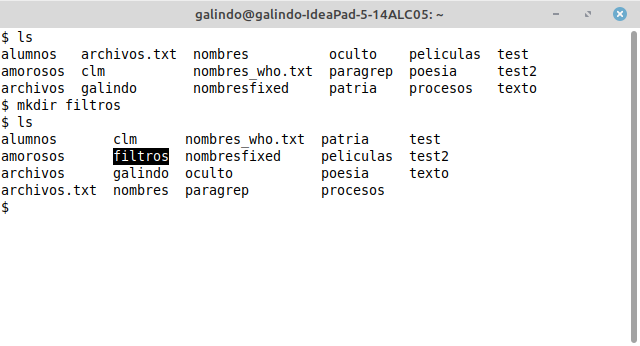
\includegraphics[width=10cm]{img/a1.png}
\caption{Directorio creado}
\end{figure}

\subsection{Eliminar todos los permisos de este directorio, dejando solo permisos para ti}
\label{sec:org6205695}
\begin{verbatim}
chmod 700 filtros
\end{verbatim}

\begin{twoc}
\begin{center}
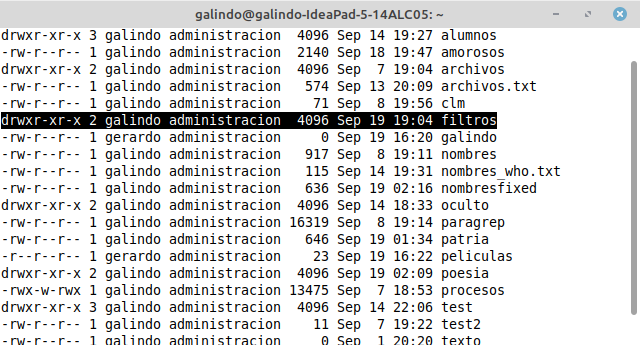
\includegraphics[width=.9\linewidth]{img/a2a.png}
\end{center}
\end{twoc}
\begin{twoc}
\begin{center}
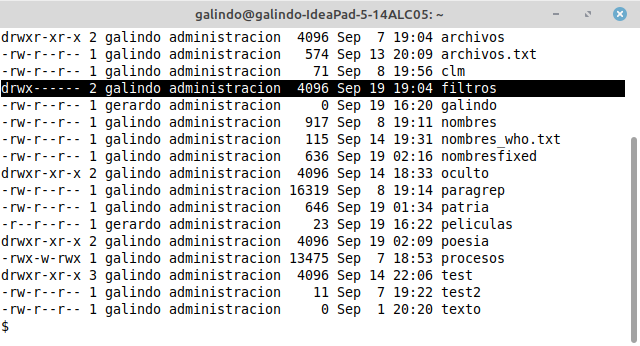
\includegraphics[width=.9\linewidth]{img/a2b.png}
\end{center}
\end{twoc}

Permisos cambiados

\subsection{Copiar el archivo 'nombres' desde 'maestro/filtros' a tu directorio 'filtros'}
\label{sec:orgd281a81}
\begin{verbatim}
cp ../alma/nombres ./filtros
\end{verbatim}

\begin{figure}[htbp]
\centering
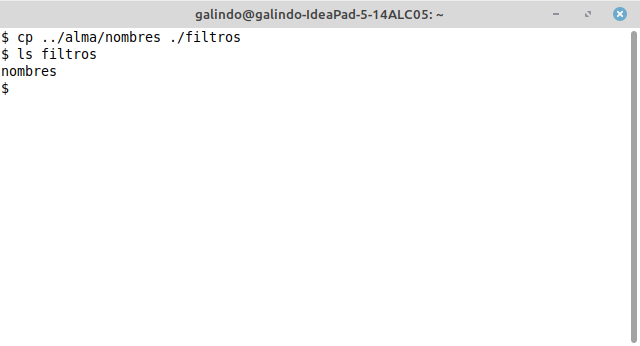
\includegraphics[width=10cm]{img/a3.png}
\caption{Archivo copiado}
\end{figure}

\pagebreak

\subsection{Mostrar el archivo 'nombres' ordenado alfabéticamente ascendente por apellido materno}
\label{sec:org0f2da5d}
\begin{verbatim}
sort -t' ' -k2 filtros/nombres
\end{verbatim}

\begin{figure}[htbp]
\centering
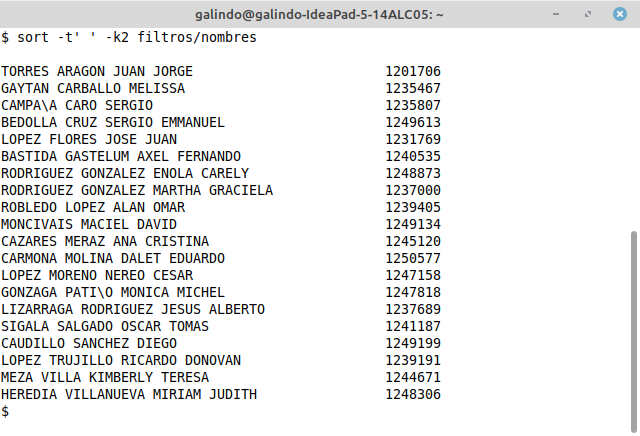
\includegraphics[width=10cm]{img/a4.png}
\caption{Archivo ordenado alfabéticamente}
\end{figure}

\cite{sort}

\subsection{Copiar el archivo 'matriculas' desde 'maestro' a tu directorio 'filtros'}
\label{sec:org2de80ad}
\begin{verbatim}
cp ../../sist20232/lety/filtros/matriculas filtros/matriculas
\end{verbatim}

\begin{figure}[htbp]
\centering
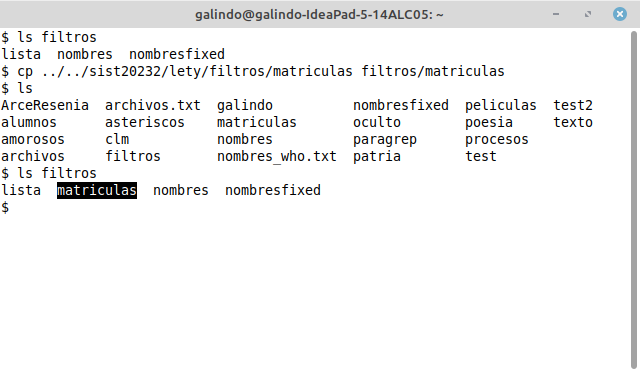
\includegraphics[width=10cm]{img/a5.png}
\caption{Archivo copia do desde matriculas a filtros}
\end{figure}

\pagebreak

\subsection{Ordenar el archivo 'matriculas' por el apellido materno}
\label{sec:org0ab71cd}
\begin{verbatim}
sort -t' ' -k4 filtros/matriculas
\end{verbatim}

\begin{figure}[htbp]
\centering
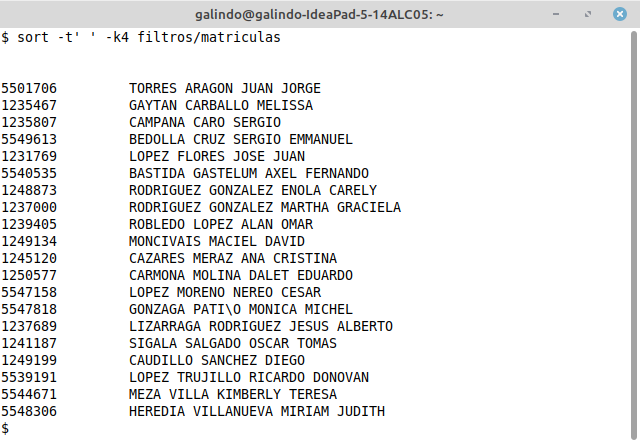
\includegraphics[width=10cm]{img/a6.png}
\caption{Salida de sort sobre matriculas}
\end{figure}

\cite{sort}

\subsection{Ordenar el archivo 'nombresfixed' por matrícula}
\label{sec:org8dacc69}
\begin{verbatim}
sort -t' ' -k4 filtros/nombresfixed
\end{verbatim}

\begin{figure}[htbp]
\centering
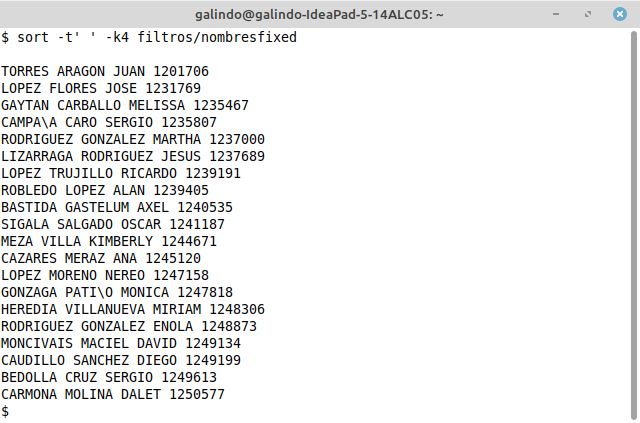
\includegraphics[width=10cm]{img/a7.png}
\caption{Ordenado por matricula}
\end{figure}

\cite{sort}

\subsection{¿Qué hace el comando \texttt{sort -f <archivo>}? (Lea el manual en línea}
\label{sec:orgaf72dcf}
\begin{mdframed}
\begin{itemize}
\item Ordena el contenido del archivo sin importar si son mayusculas o minusculas
\end{itemize}
\end{mdframed}

\cite{sort}

\subsection{Ordenar el archivo 'matriculas' en forma descendente por apellido paterno}
\label{sec:org7ad40e5}
\begin{verbatim}
sort -t' ' -k1r filtros/nombresfixed
\end{verbatim}

\begin{figure}[htbp]
\centering
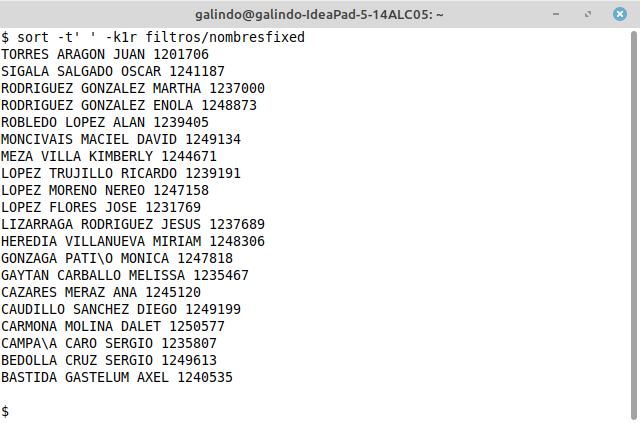
\includegraphics[width=10cm]{img/a9.png}
\caption[\texttt{-r}]{La columna 1 representa el apellido paterno \texttt{-r} cambia al orden inverso}
\end{figure}

\subsection{Copiar el archivo 'delim' a tu directorio 'filtros'}
\label{sec:org6cae7f7}
\begin{verbatim}
cp ../alma/delim filtros/
\end{verbatim}

\begin{figure}[htbp]
\centering
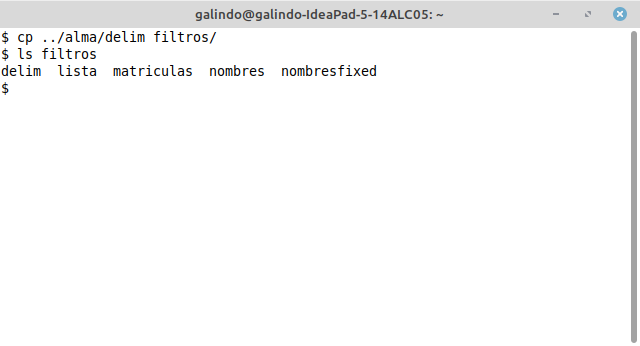
\includegraphics[width=10cm]{img/a10.png}
\caption[\texttt{../alma}]{Achivo delim copiado desde el directorio \texttt{../alma}}
\end{figure}

\subsection{Copiar el archivo 'lista' desde 'maestro/filtros' a tu directorio 'filtros'}
\label{sec:org2008b44}
\begin{verbatim}
cp ../alma/lista ~/filtros/
\end{verbatim}

\begin{figure}[htbp]
\centering
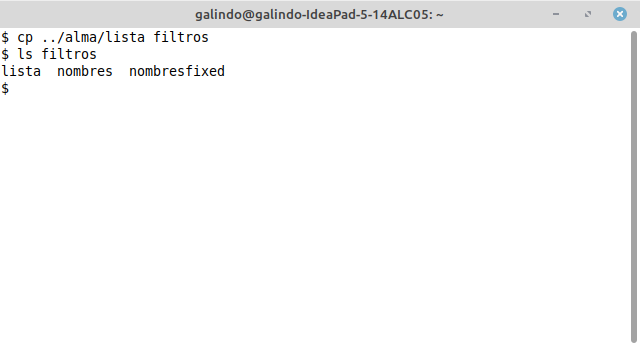
\includegraphics[width=10cm]{img/a11.png}
\caption{Archivo lsita copiado}
\end{figure}

\subsection{Ordenar el archivo 'matriculas' en forma numérica descendente}
\label{sec:org110e58d}
\begin{verbatim}
sort -t' ' -k4r filtros/nombresfixed
\end{verbatim}

\begin{figure}[htbp]
\centering
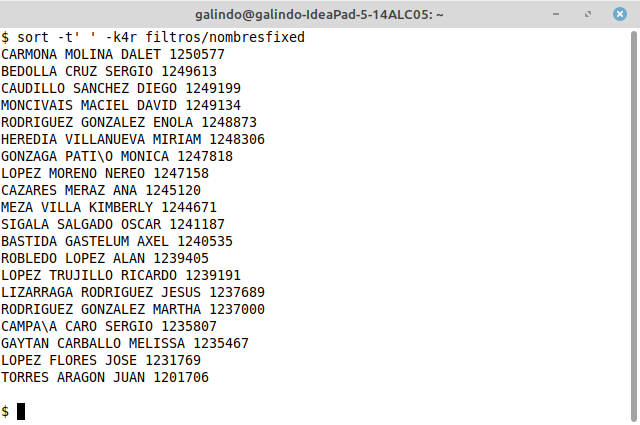
\includegraphics[width=10cm]{img/a13.png}
\caption{Ordenamiento por matriculas}
\end{figure}

\pagebreak

\subsection{Ordenar el archivo 'nombres' por nombre en forma descendente}
\label{sec:org54ad78b}
\begin{verbatim}
sort -t' ' -k3r filtros/nombres
\end{verbatim}

\begin{figure}[htbp]
\centering
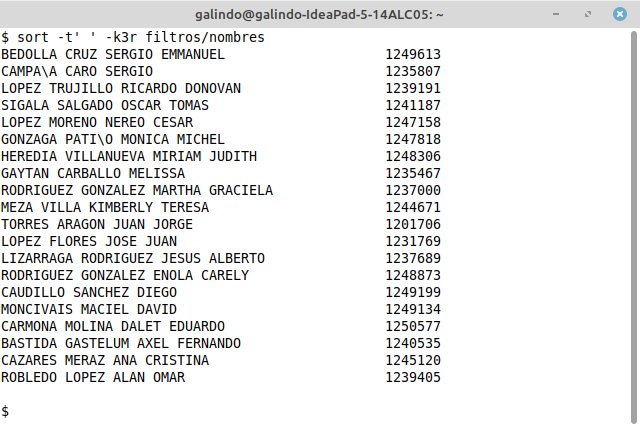
\includegraphics[width=10cm]{img/a14.png}
\caption{Ordenado por nombres de manera descendiente}
\end{figure}

\subsection{Mostrar la primera y última columna del archivo 'asteriscos'}
\label{sec:org332f9cf}
\begin{verbatim}
cut -d'*' -f1,3 asteriscos
\end{verbatim}

\begin{figure}[htbp]
\centering
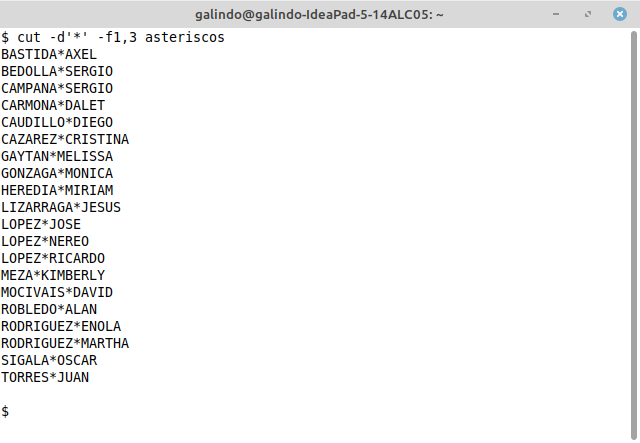
\includegraphics[width=10cm]{img/a14b.png}
\caption{Separador reemplazado por '*'}
\end{figure}

\subsection{*Contar cuántos alumnos se llaman Jesús en los archivos 'lista' y 'nombres' y compara los números}
\label{sec:org1d7b877}
\subsection{Mostrar a todos los alumnos cuya matrícula empiece con '12' en el archivo 'nombres'}
\label{sec:org5d783ce}
\begin{verbatim}
grep "^12" filtros/matriculas
\end{verbatim}

\begin{figure}[htbp]
\centering
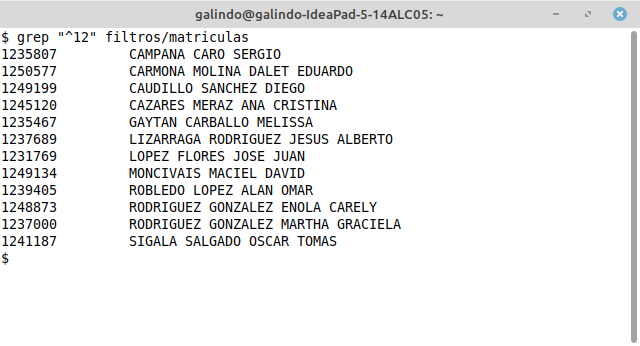
\includegraphics[width=10cm]{img/a16.png}
\caption{se reemplazó '55' por '12' para que mostrara resultados}
\end{figure}

\subsection{Contar las líneas en el archivo 'hormigas'}
\label{sec:orgc21f77b}
\begin{itemize}
\item el archivo tiene 37 lineas
\end{itemize}

\begin{verbatim}
wc -l ../alma/hormigas
\end{verbatim}

\begin{figure}[htbp]
\centering
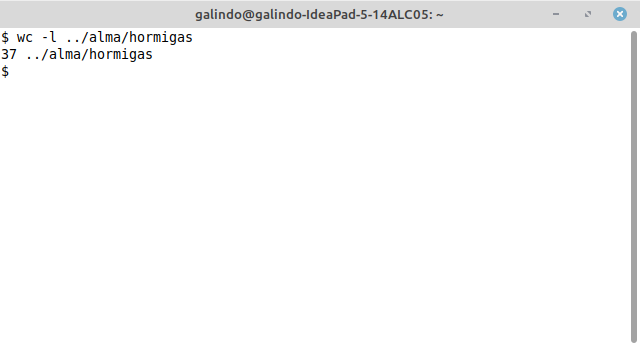
\includegraphics[width=10cm]{img/a17.png}
\caption[\texttt{wc}]{Salida de \texttt{wc}}
\end{figure}

\pagebreak

\subsection{Buscar la frase 'las hormigas' en el archivo 'hormigas' y mostrar las líneas donde aparece}
\label{sec:org6a32e06}
\begin{verbatim}
grep -n "las hormigas" ../alma/hormigas
\end{verbatim}

\begin{figure}[htbp]
\centering
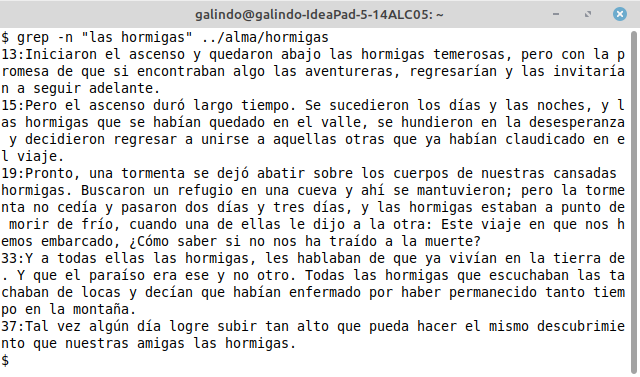
\includegraphics[width=10cm]{img/a18.png}
\caption{'as hormigas' aparecen varias veces en el texto}
\end{figure}

\subsection{Mostrar solo las líneas que comienzan con 'La' en el archivo 'hormigas'}
\label{sec:org3147b7b}
\begin{verbatim}
grep -n "^La" ../alma/hormigas
\end{verbatim}

\begin{figure}[htbp]
\centering
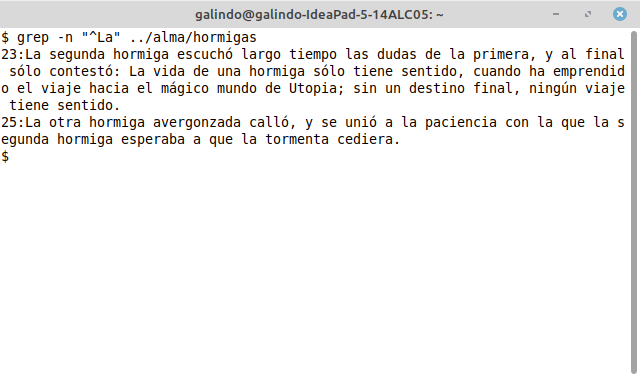
\includegraphics[width=10cm]{img/a19.png}
\caption[\texttt{grep}]{\texttt{grep} nos ayuda a encontrar las veces que aparece}
\end{figure}

\pagebreak

\subsection{*Mostrar a los alumnos que tienen un nombre o apellido de cuatro letras en el archivo 'lista'}
\label{sec:orgf187978}
\subsection{Mostrar a los alumnos que no se apellidan "Perez" en el archivo 'lista'}
\label{sec:org01dff0a}
\begin{verbatim}
grep -v "Perez" lista
\end{verbatim}

\begin{figure}[htbp]
\centering
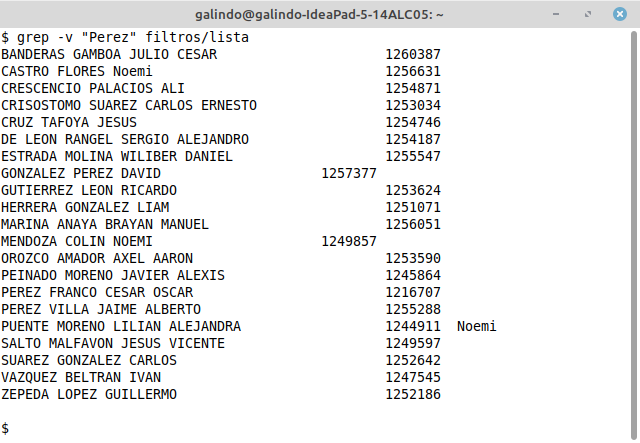
\includegraphics[width=10cm]{img/21.png}
\caption[\texttt{-v}]{\texttt{-v} muestra las lineas que no contienen el string}
\end{figure}

\subsection{Mostrar solo el nombre y apellido del archivo 'delim'}
\label{sec:orgab2300a}
\begin{verbatim}
cut -d':' -f2,3 ../alma/delim
\end{verbatim}

\begin{figure}[htbp]
\centering
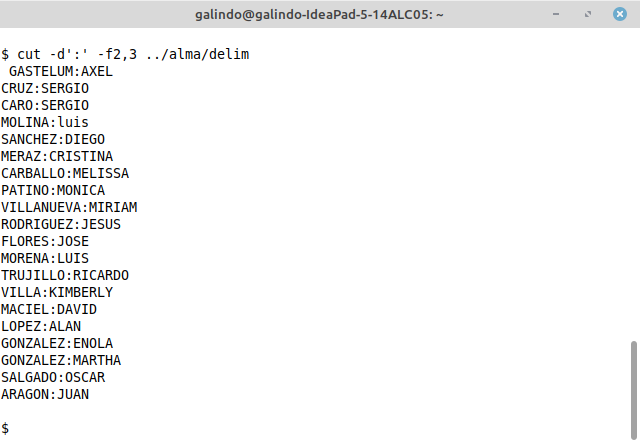
\includegraphics[width=10cm]{img/a22.png}
\caption[\texttt{-f2,3}]{\texttt{-d} cambia el separado y \texttt{-f2,3} nos muestra las columnas 2 y 3}
\end{figure}

\subsection{Mostrar solo las matrículas del archivo 'delim'}
\label{sec:org543400b}
\begin{verbatim}
cut -d':' -f4 ../alma/delim
\end{verbatim}

\begin{figure}[htbp]
\centering
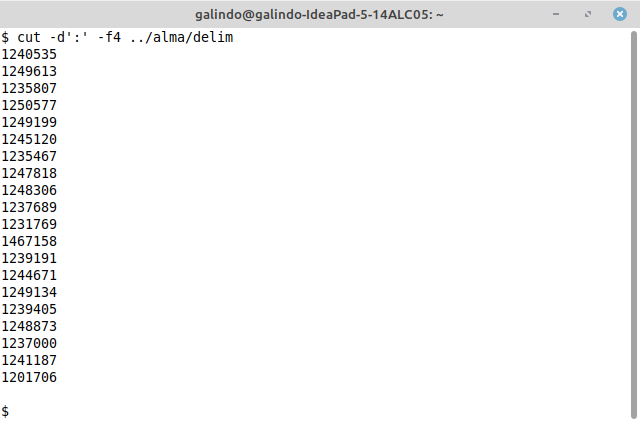
\includegraphics[width=10cm]{img/a23.png}
\caption{Cortamos la columna 4 del archivo}
\end{figure}

\subsection{Mostrar solo la primera columna de caracteres del archivo 'lista'}
\label{sec:org07156b8}
\begin{verbatim}
cut -c1 ../alma/lista
\end{verbatim}

\begin{figure}[htbp]
\centering
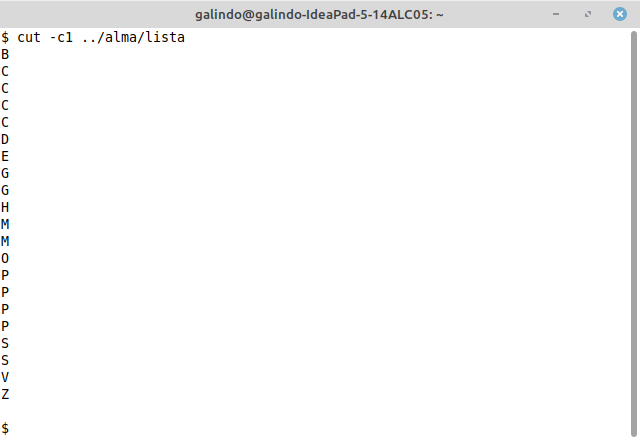
\includegraphics[width=10cm]{img/a24.png}
\caption[\texttt{-c}]{\texttt{-c} extrae la primer columna de caracteres}
\end{figure}

\pagebreak

\subsection{Mostrar los caracteres 18 al 25 del archivo 'hormigas'}
\label{sec:org2c2864a}
\begin{verbatim}
cut -c18-25 ../alma/hormigas
\end{verbatim}

\begin{figure}[htbp]
\centering
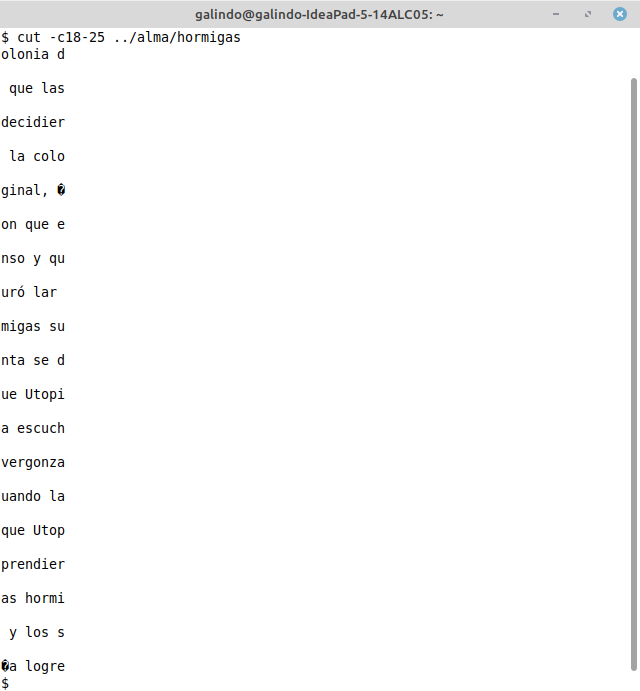
\includegraphics[width=10cm]{img/a25.png}
\caption[\texttt{-c18-25}]{\texttt{-c} extrae caracteres \texttt{-c18-25} limita el rango}
\end{figure}

\pagebreak

\subsection{Mostrar el campo número 3 del archivo 'delim'}
\label{sec:orga970066}
\begin{verbatim}
cut -d':' -f3 ../alma/delim
\end{verbatim}

\begin{figure}[htbp]
\centering
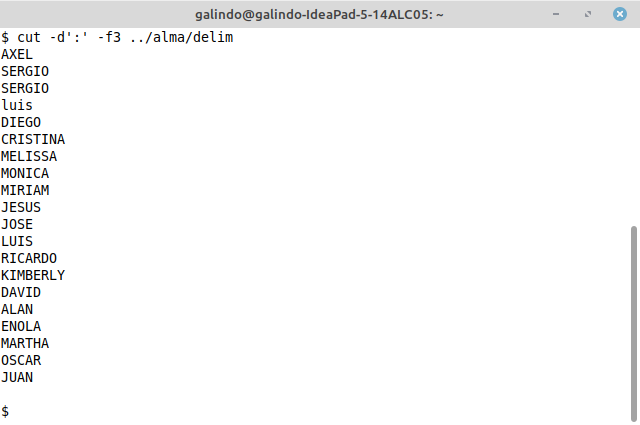
\includegraphics[width=10cm]{img/a26.png}
\caption[\texttt{-f3}]{\texttt{-d} cambia el delimitador y \texttt{-f3} selecciona la columna}
\end{figure}

\subsection{Mostrar las líneas del archivo 'lista' donde el apellido paterno sea 'Perez'}
\label{sec:org143d236}
\begin{verbatim}
grep -n "PEREZ" ../alma/lista
\end{verbatim}

\begin{figure}[htbp]
\centering
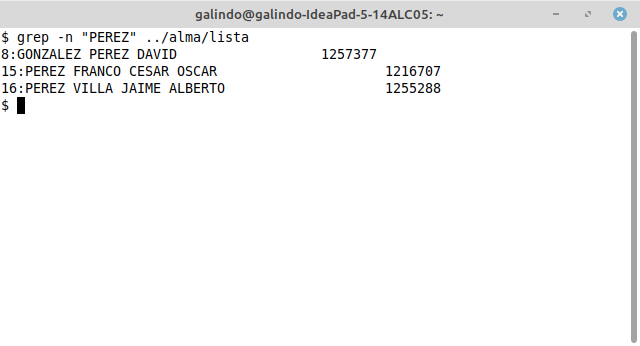
\includegraphics[width=10cm]{img/a27.png}
\caption[\texttt{grep}]{el flag \texttt{-n} en \texttt{grep} agrega el numero de linea en el archivo}
\end{figure}


\pagebreak

\subsection{Mostrar las líneas del archivo 'delim' cuyo nombre sea 'luis'}
\label{sec:org90bbed8}
\begin{verbatim}
grep "luis" ../alma/delim
\end{verbatim}

\begin{figure}[htbp]
\centering
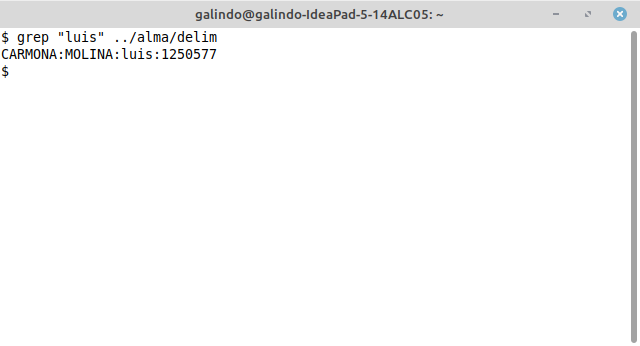
\includegraphics[width=10cm]{img/a28.png}
\caption[\texttt{grep}]{Salida de \texttt{grep} ''luis''}
\end{figure}

\subsection{Mostrar las líneas del archivo 'hormigas' que contienen la palabra 'Utopia' y mostrar sus números de línea}
\label{sec:orgfbb3ad3}
\begin{verbatim}
grep -n "Utopia" ../alma/hormigas
\end{verbatim}

\begin{figure}[htbp]
\centering
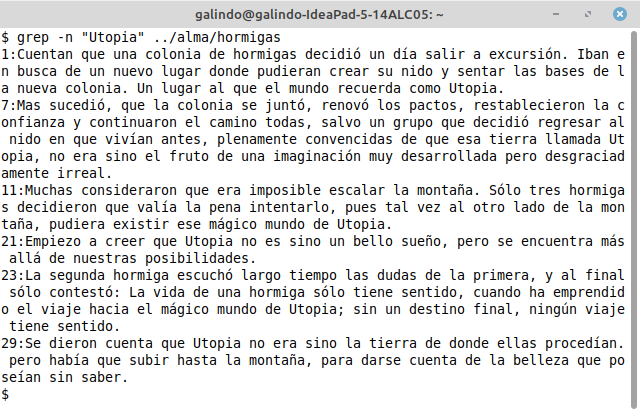
\includegraphics[width=10cm]{img/a29.png}
\caption[\texttt{grep}]{salida de \texttt{grep} -n ''Utopia''}
\end{figure}

\pagebreak

\subsection{Mostrar la línea del archivo 'lista' que contiene el nombre 'Noemi' al final}
\label{sec:org795825c}
\begin{verbatim}
grep " Noemi" lista
\end{verbatim}

\begin{figure}[htbp]
\centering
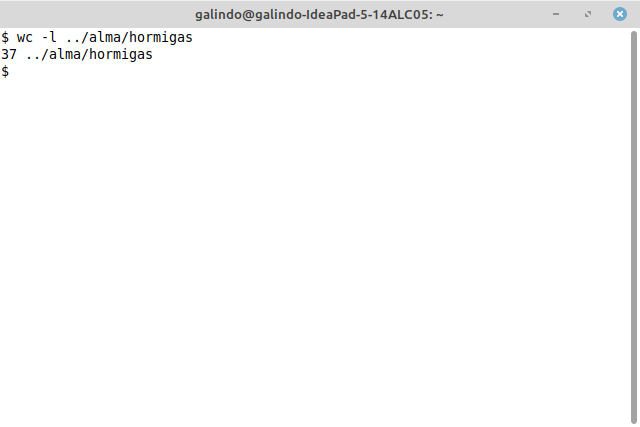
\includegraphics[width=10cm]{img/a30.png}
\caption[\texttt{grep}]{salida de \texttt{grep} '' Noemi'' lista}
\end{figure}

\subsection{Mostrar las líneas del archivo 'hormigas' que contienen las palabras 'hormigos' o 'hormigas'}
\label{sec:org581ed24}
\begin{verbatim}
grep -E "hormigos|hormigas" ../alma/hormigas
\end{verbatim}

\begin{figure}[htbp]
\centering
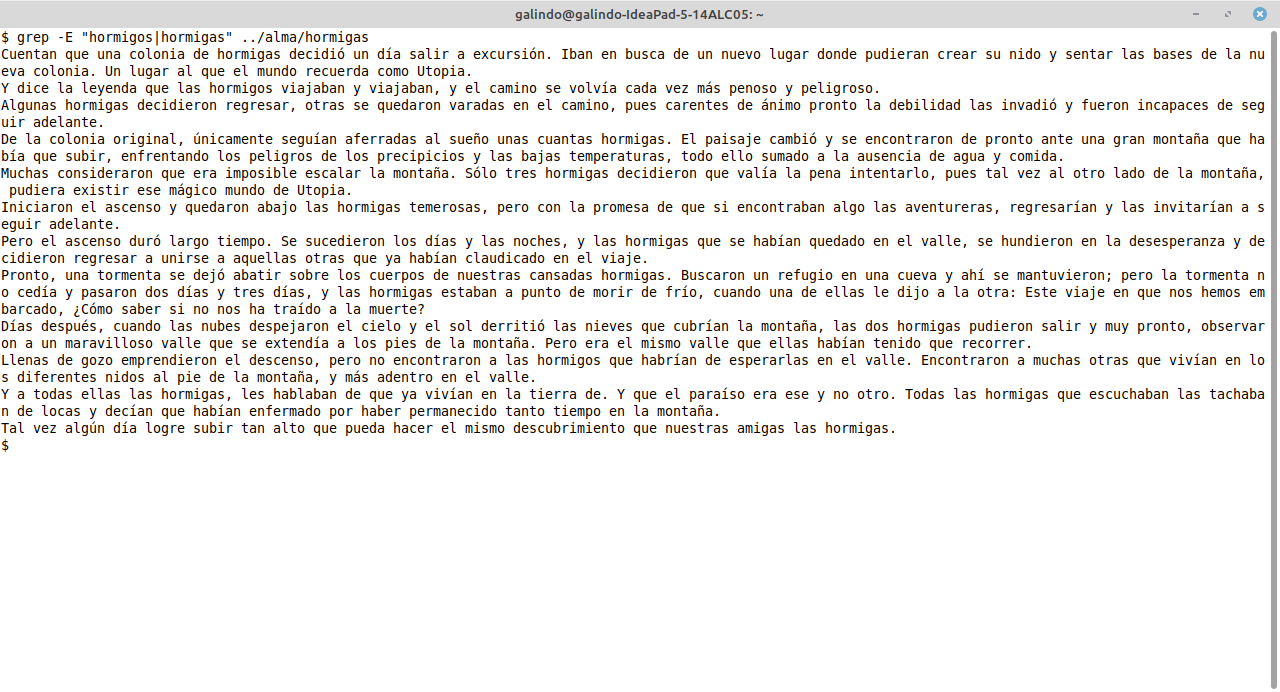
\includegraphics[width=10cm]{img/a31.png}
\caption{}
\end{figure}

\cite{man7}

\pagebreak

\subsection{Mostrar las líneas en el archivo 'asteriscos' que no empiezan con 'F', 'G' o 'H'}
\label{sec:orgced1ffd}
\begin{verbatim}
grep -v "^[FGH]" asteriscos
\end{verbatim}

\begin{figure}[htbp]
\centering
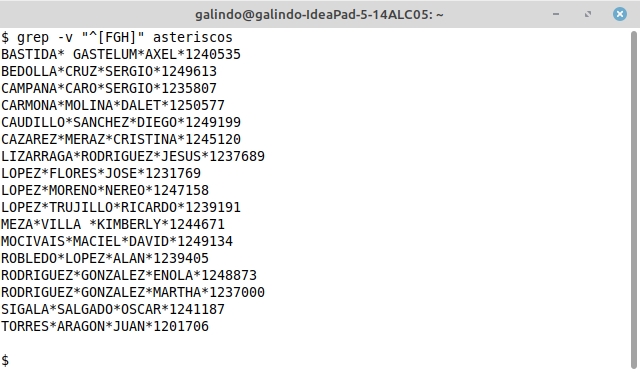
\includegraphics[width=10cm]{img/a32.png}
\caption{}
\end{figure}


\section{Conclusión}
\label{sec:orgbda165a}
A lo largo de esta practica aprendí a como buscar información dentro de ficheros
separar por columnas, compara archivos y buscar texto dentro de ellos, pienso que 
conocer estas cosas sera de muchas importancia ya que al no contar con una 
interfaz gráfica esto se permitiría simplificar el proceso.

\section{Referencias}
\label{sec:orgf359461}
\printbibliography[heading=none]
\end{document}
